\documentclass{article}
\usepackage[utf8]{inputenc}    % For UTF-8 character encoding
\usepackage[T1]{fontenc}       % For proper font encoding
\usepackage{lmodern}           % Improved font rendering
\usepackage{amsmath}   % For advanced mathematical formatting
\usepackage{amssymb}   % For mathematical symbols
\usepackage{geometry}  % Adjust page margins
\usepackage{enumerate} % For custom lists
\usepackage{xcolor}  % for coloring
\usepackage{amsthm}
\usepackage{pdfpages}
\newtheorem{theorem}{Theorem}[section]
\newtheorem{lemma}[theorem]{Lemma}
\newtheorem{corollary}[theorem]{Corollary}
\newtheorem{definition}[theorem]{Definition}
\usepackage{listings}  % for code listings
\usepackage{tikz}
\usetikzlibrary{er}  % for ER diagram shapes
\tikzset{
  link/.style={-} % a simple straight line
}

\lstset{frame=tb,
  language=C,
  aboveskip=3mm,
  belowskip=3mm,
  showstringspaces=false,   
  columns=flexible,
  basicstyle={\small\ttfamily},
  numbers=none,
  numberstyle=\tiny\color{gray},
  keywordstyle=\color{blue},
  commentstyle=\color{brown},
  stringstyle=\color{orange},
  breaklines=true,
  breakatwhitespace=true,
  tabsize=3
}
\geometry{top=1in, bottom=1in, left=1in, right=1in}

\begin{document}

\title{}
\author{Wang Xiyu}
\date{}
\maketitle


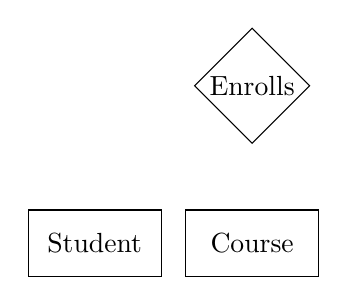
\begin{tikzpicture}[node distance=2cm, every edge/.style={link}]
  % Entities
  \node[entity] (student) {Student};
  \node[entity, right of=student] (course) {Course};

  % Relationship
  \node[relationship, above of=course] (enrolls) {Enrolls};

  % Connect
  \path (student) edge (enrolls)
        (course) edge (enrolls);
\end{tikzpicture}


\end{document}